\chapter{Appendix 1} \label{app1}

\section{Comparing ngram size} \label{ngram}

Here we are comparing the average accuracy across 10 folds of using different ngram size ranges. We include two different classifiers.

\begin{figure}[H]
\center
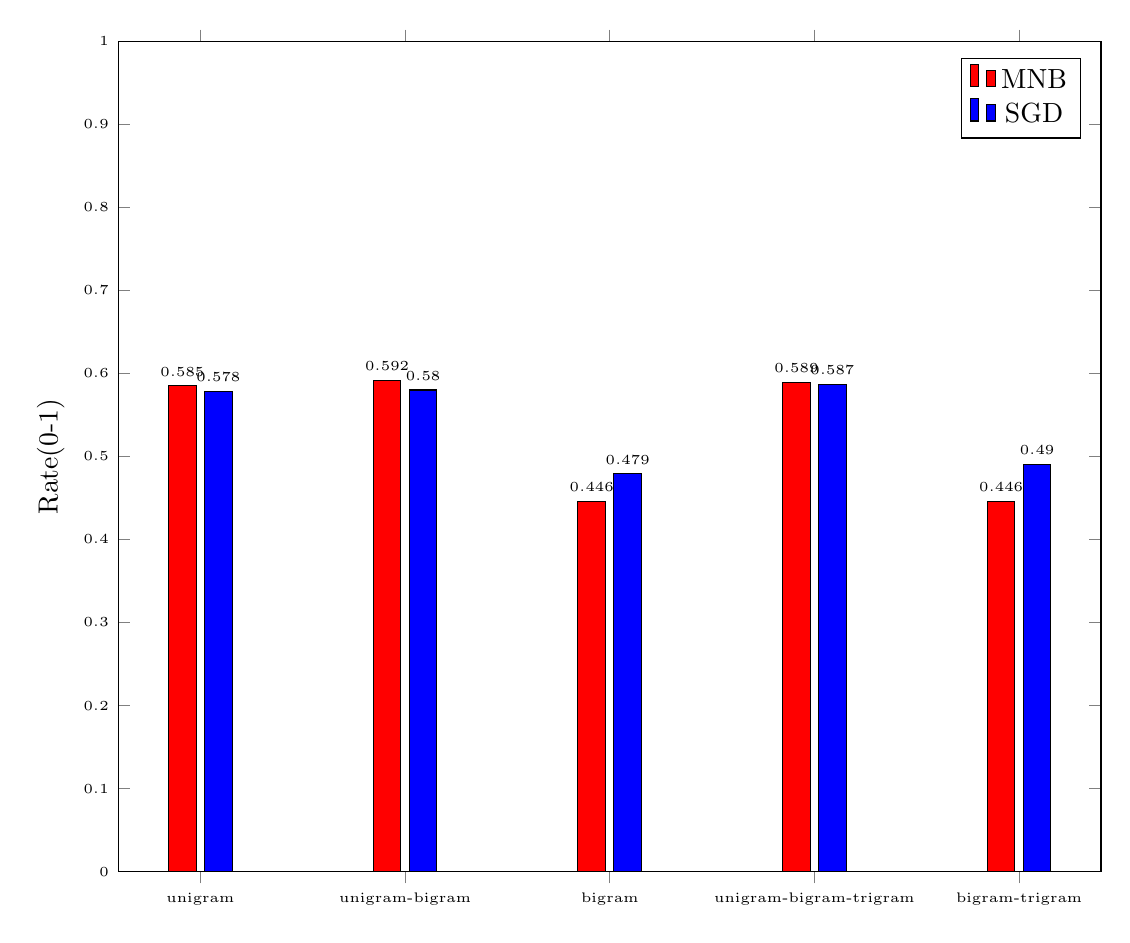
\begin{tikzpicture}
\begin{axis}[
	ymin = 0,
	ymax = 1,
	width = 400,
	symbolic x coords={unigram,unigram-bigram,bigram,unigram-bigram-trigram,bigram-trigram},
    xtick=data,
	ylabel=Rate(0-1),
	compat=newest, %Better label placement,
	ybar = 3,
	nodes near coords,
	scaled x ticks = false,
	tick label style={font=\tiny} ,
	every node near coord/.append style={/pgf/number format/fixed, /pgf/number format/precision=3, font=\fontsize{1}{1}\selectfont},
]


\addplot [ybar, fill=red]
	coordinates {
		(unigram,0.585) (unigram-bigram,0.592)
		 (bigram,0.446) (unigram-bigram-trigram,0.589) (bigram-trigram, 0.446)
		 
		 };
		 
		 
\addplot [ybar, fill=blue]
	coordinates {
		(unigram,0.578) (unigram-bigram,0.580)
		 (bigram,0.479) (unigram-bigram-trigram,0.587) (bigram-trigram, 0.490)
		 
		 };
		 
		 				 	
\addlegendentry{MNB}
\addlegendentry{SGD}
\title{F-Measure Rates}
\end{axis}
\end{tikzpicture}
\caption{Comparison of average accuracy between ngram ranges across 10 folds}
\end{figure}


\section{Comparing df} \label{df}

Here we are comparing minimum document frequency and the average system accuracy that results.

\begin{figure}[H]
\center
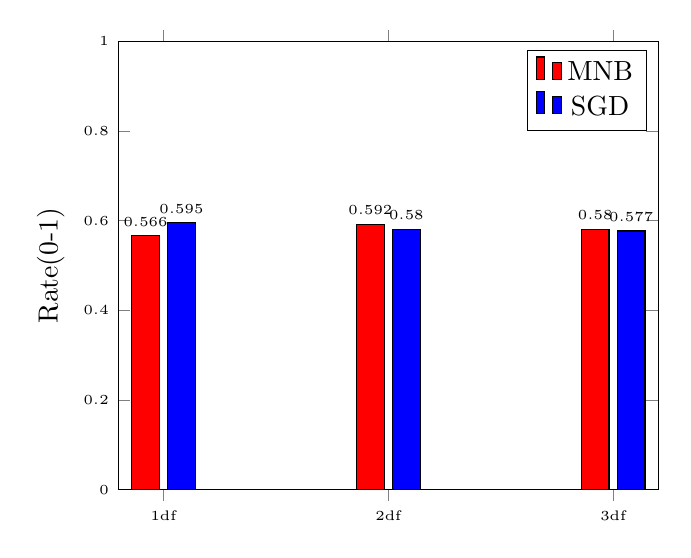
\begin{tikzpicture}
\begin{axis}[
	ymin = 0,
	ymax = 1,
	symbolic x coords={1df,2df,3df},
    xtick=data,
	ylabel=Rate(0-1),
	compat=newest, %Better label placement,
	ybar = 3,
	nodes near coords,
	scaled x ticks = false,
	tick label style={font=\tiny} ,
	every node near coord/.append style={/pgf/number format/fixed, /pgf/number format/precision=3, font=\fontsize{1}{1}\selectfont},
]


\addplot [ybar, fill=red]
	coordinates {
		(1df, 0.566) (2df,0.592)
		 (3df,0.580) 
		 
		 };
		  
\addplot [ybar, fill=blue]
	coordinates {
		(1df,0.595) (2df,0.580)
		 (3df,0.577)
		 
		 };
		 
		 				 	
\addlegendentry{MNB}
\addlegendentry{SGD}
\title{F-Measure Rates}
\end{axis}
\end{tikzpicture}
\caption{Comparison of average accuracy between df threshold across 10 folds}
\end{figure}


\section{Full Comparison of Stemmers and Lemmatizers} \label{comp_stem}

\begin{figure}[H]
\center
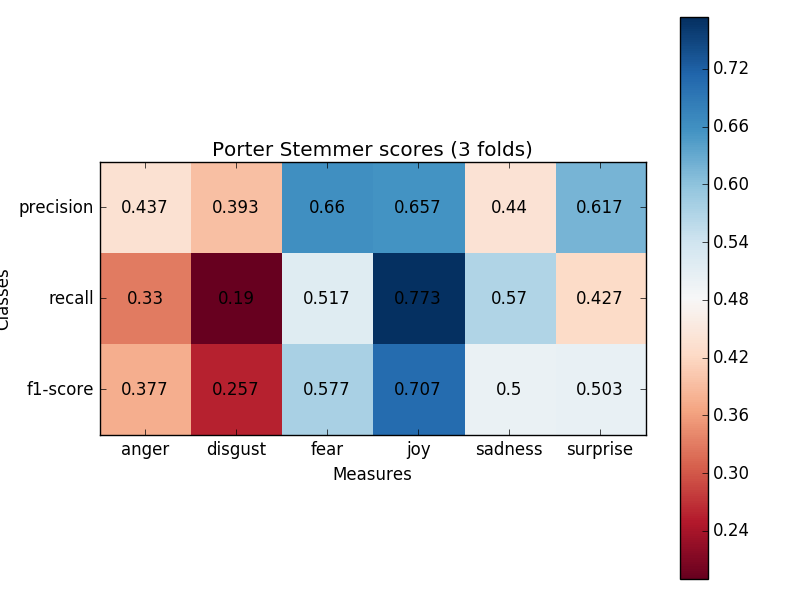
\includegraphics[width=12cm]{images/porter_matrix.png}
\caption{Confusion Matrix for Porter Stemmer}
\end{figure}


\begin{figure}[H]
\center
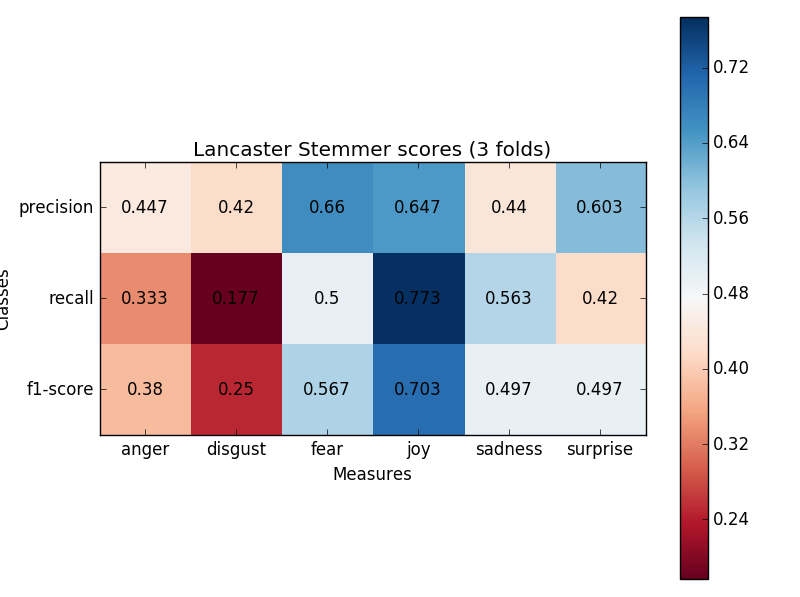
\includegraphics[width=12cm]{images/Lancaster_matrix.png}
\caption{Confusion Matrix for Lancaster Stemmer}
\end{figure}

\begin{figure}[H]
\center
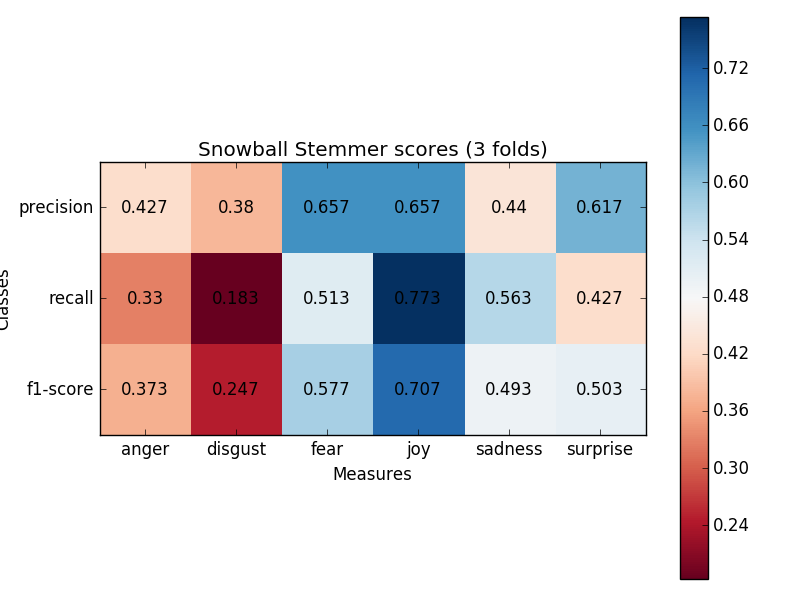
\includegraphics[width=12cm]{images/Snowball_matrix.png}
\caption{Confusion Matrix for Snowball Stemmer}
\end{figure}

\begin{figure}[H]
\center
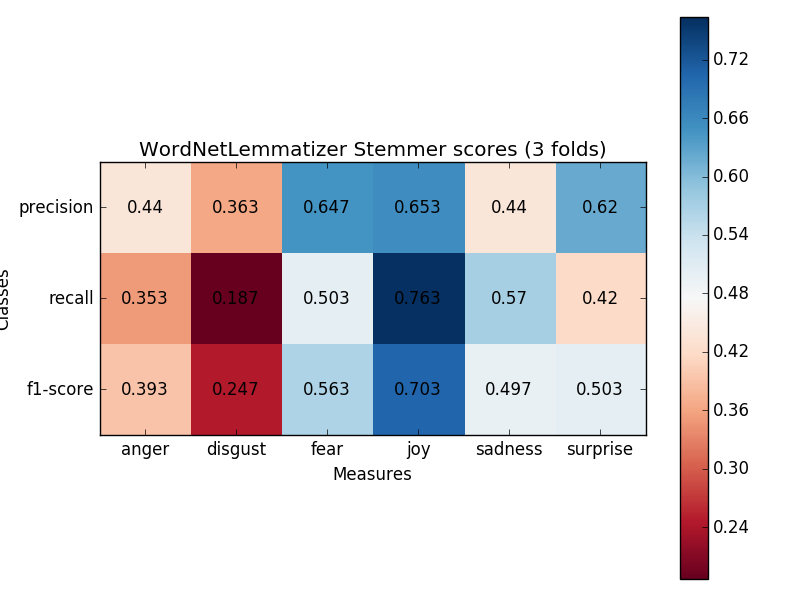
\includegraphics[width=12cm]{images/WordNetLemmatizer_matrix.png}
\caption{Confusion Matrix for WordNetLemmatizer}
\end{figure}
